% Created 2016-05-24 Tue 17:09
\documentclass[11pt,xcolor=dvipsnames,presentation]{beamer}
\usepackage[utf8]{inputenc}
\usepackage[T1]{fontenc}
\usepackage{fixltx2e}
\usepackage{graphicx}
\usepackage{longtable}
\usepackage{float}
\usepackage{wrapfig}
\usepackage{rotating}
\usepackage[normalem]{ulem}
\usepackage{amsmath}
\usepackage{textcomp}
\usepackage{marvosym}
\usepackage{wasysym}
\usepackage{amssymb}
\usepackage{hyperref}
\tolerance=1000
\usepackage{minted}
\PassOptionsToPackage{svgnames}{xcolor}
\let\AtBeginDocumentSav=\AtBeginDocument
\def\AtBeginDocument#1{}
\input{org-babel-style-preembule.tex}
\let\AtBeginDocument=\AtBeginDocumentSav
\usepackage{minted}
\usepackage{multirow}
\usetikzlibrary{arrows,shapes,positioning}
\usepackage{subcaption}
\let\tmptableofcontents=\tableofcontents
\def\tableofcontents{}
\usepackage{color,soul}
\definecolor{lightblue}{rgb}{1,.9,.7}
\sethlcolor{lightblue}
\let\hrefold=\href
\renewcommand{\href}[2]{\hrefold{#1}{\SoulColor\hl{#2}}}
\newcommand{\muuline}[1]{\SoulColor\hl{#1}}
\makeatletter
\newcommand\SoulColor{%
\let\set@color\beamerorig@set@color
\let\reset@color\beamerorig@reset@color}
\makeatother
\newcommand{\bottomcitepre}[1]{\fbox{\vbox{\footnotesize #1}}}
\def\mylogos{\\\vspace{1cm}\begin{center}\includegraphics[height=1.2cm]{logos/inr_logo_sans_sign_coul.png}\hspace{0.5cm}\insertlogo{\includegraphics[height=1.2cm]{logos/grid5000.png}}\hspace{0.5cm}\end{center}\vspace{-1cm}}
\usetheme{default}
\usecolortheme{}
\usefonttheme{}
\useinnertheme{}
\useoutertheme{}
\author{Cristian Ruiz \\ \vspace{0.5cm} MADYNES Team}
\date{May 31, 2016 --  young engineers seminar \mylogos}
\title{ADT COSETTE}
\hypersetup{
  pdfkeywords={},
  pdfsubject={},
  pdfcreator={Emacs 24.3.1 (Org mode 8.2.10)}}
\begin{document}

\maketitle


\section{}
\label{sec-1}
\begin{frame}[label=sec-1-0-1]{Validation in Computer Science}
Two classical approaches for validation:

\begin{itemize}
\item \alert{Formal:} equations, proofs, etc.
\item \alert{Experimental}, on a scientific instrument.
\end{itemize}

\begin{block}{In reality}
Given the size and complexity of distributed systems,
it is difficult to carry out complete analytic studies.
\alert{So, the experimental approach is commonly seen}.
\end{block}

\begin{block}{Need of}
\alert{Reproducible research}
\end{block}
\end{frame}

\begin{frame}[label=sec-1-0-2]{Grid'5000}
A large-scale, shared testbed supporting high-quality,
reproducible research on distributed systems:

\begin{itemize}
\item Highly configurable
\item High Performance Computing, Grids, Peer-to-peer systems, Cloud computing
\end{itemize}

Another examples of testbeds: Chameleon, Cloudlab
\begin{columns}
\begin{column}{0.5\textwidth}

\begin{figure}[!h]
  \center
  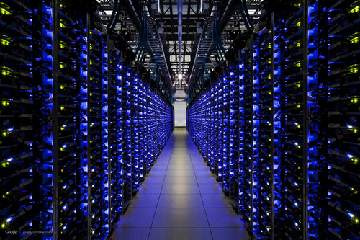
\includegraphics[scale=0.33]{figures/hpc.png}
  \label{fig:hpc}
\end{figure}
\end{column}
\end{columns}
\end{frame}


\begin{frame}[label=sec-1-0-3]{Goal of the ADT COSETTE}
Conceive, consolidate and extend a set of tools
aimed at experimenting with distributed systems
(Cloud, Grid, HPC, P2P)

\begin{block}{Tasks}
\begin{itemize}
\item Development of Ruby-Cute, a library that gathers useful
procedures for experimenting with distributed systems
\item \alert{Extend Distem to meet Cloud and HPC research requirements}
\end{itemize}
\end{block}


\begin{block}{Supervised by}
Lucas Nussbaum, Emmanuel Jeanvoine
\end{block}
\end{frame}



\section{Distem}
\label{sec-2}
\let\tableofcontents=\tmptableofcontents
\AtBeginSection[]
  {
     \begin{frame}<beamer>
     \frametitle{Outline}
     \tableofcontents[currentsection]
     \end{frame}
  }
\input{org-babel-document-preembule.tex}

\begin{frame}[label=sec-2-0-1]{Distem}
\begin{center}
\huge
An emulator for distributed systems\\[0.5em]
\large
Take your \alert{real application}\\[0.5em]
Run it on a \alert{cluster}\\[0.5em]
And use \alert{Distem} to \alert{alter the platform}\\
so it \alert{matches the experimental conditions you need}\\[1em]
\normalsize
\begin{tikzpicture}
\pgftext[right]{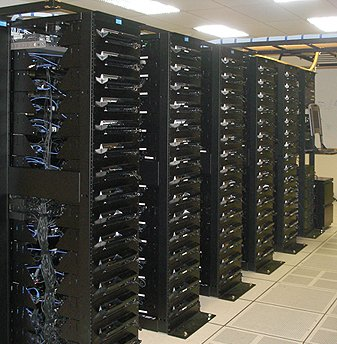
\includegraphics[width=3cm]{figures/cluster.jpg}}
\draw[line width=1.5mm] (0.1, 0) -- (0.9, 0);
\draw[line width=1.5mm] (0.5, -0.4) -- (0.5, 0.4);
\pgftext[x=1.25cm,left]{
\includegraphics[width=2.5cm]{figures/distem.png}}
\draw[line width=1.5mm,->] (4.1,0) -> (4.9,0);
\begin{scope}[xshift=2cm]
\pgftext[x=5cm,y=0.75cm,center]{Heterogeneous nodes}
\pgftext[x=5cm,y=0.25cm,center]{Long distance networks}
\pgftext[x=5cm,y=-0.25cm,center]{Faults, perf. variations}
\pgftext[x=5cm,y=-0.75cm,center]{Grid, Cloud, P2P features}
\pgftext[x=5cm,y=-1.25cm,center]{\Large\ldots}
\end{scope}
\end{tikzpicture}
\end{center}
\end{frame}

\begin{frame}[label=sec-2-0-2]{Distem features}
The features of Distem include:

\begin{itemize}
\item running many virtual nodes on each physical node
\item emulation of CPU performance, network topologies, I/O speed
\end{itemize}

Distem uses modern Linux functionality:

\begin{itemize}
\item Linux containers
\item control groups
\item CPU frequency scaling
\item traffic control
\item I/O throttling
\end{itemize}
\end{frame}



\section{Evaluating HPC runtimes with Distem}
\label{sec-3}
\begin{frame}[label=sec-3-0-1]{HPC runtimes}
\begin{itemize}
\item According to the IESP report a strong effort must be made on improving HPC software stacks
\item One of the main parts of this stack is dedicated to \alert{HPC runtime}
\item HPC runtime enables the execution, managing and debugging of parallel applications
\item OpenMPI, Charm++, CUDA, etc.
\end{itemize}


\alert{For this work we focus on studying HPC runtimes}

\vspace{1cm}
\bottomcitepre{Dongarra, Jack \textit{et Al.},
  {\textit{The International Exascale Software Project Roadmap}},
  International Journal of High Performance Computer Applications, 2011}
\end{frame}

\begin{frame}[label=sec-3-0-2]{Evaluating current HPC runtimes}
\begin{block}{Several properties to evaluate}
\begin{itemize}
\item Programmability
\item Scalability
\item \alert{Fault tolerance}
\item \alert{Load balancing}
\end{itemize}
\end{block}

\begin{block}{We focus on}
\begin{itemize}
\item Fault tolerance:
more components $\Rightarrow$ shorter MTBF \newline
(Mean Time Between Failures)

\item Load balancing: Cloud computing, Green computing, \newline
  Data centers' policies
\end{itemize}
\end{block}
\end{frame}


\begin{frame}[label=sec-3-0-3]{Evaluating current HPC runtimes}
\begin{itemize}
\item Carrying out evaluation under complex realistic conditions is \alert{hard}
\item Simulator:
\begin{itemize}
\item simplified assumptions $\frowny$
\item lower realism $\frowny$
\item not possible to run a complete software stack $\frowny$
\end{itemize}

\item Real platform:
\begin{itemize}
\item expensive $\frowny$
\item lacks of reproducibility $\frowny$
\end{itemize}
\end{itemize}
\end{frame}


\begin{frame}[label=sec-3-0-4]{In this task}
We integrated the following improvements in order to
make possible the evaluation of HPC runtimes:

\begin{itemize}
\item Evolving experimental conditions
\item Failure injection framework
\item Event injection framework
\end{itemize}
\end{frame}

\begin{frame}[label=sec-3-0-5]{Evolving experimental conditions}

\begin{minipage}{0.5\textwidth}
\begin{center}
    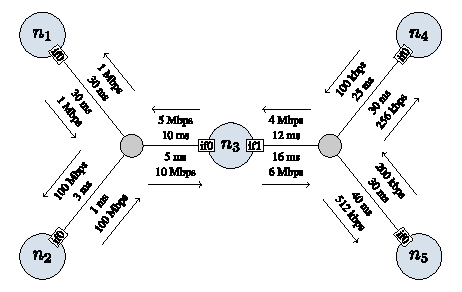
\includegraphics[width=0.9\textwidth]{figures/links}
\end{center}\end{minipage}\hfill
\begin{minipage}{0.5\textwidth}
\begin{center}
    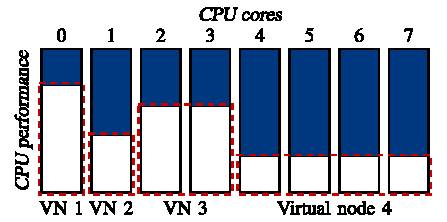
\includegraphics[width=\textwidth]{figures/procs}
\end{center}\end{minipage}

\begin{itemize}
\item Heterogeneous conditions can be created: CPU frequencies,
different IO and network capabilities

\item These features can be updated dynamically

\item This is useful to achieve complex experiments where the platform is modified,
like it could happened in reality
\end{itemize}
\end{frame}

\begin{frame}[label=sec-3-0-6]{Failure injection framework}

\begin{itemize}
\item We take into account failures that provoke a lost of the node (very common failures)

\item Nodes can be lost in three different ways:

\begin{itemize}
\item \alert{Graceful}: the node is shut down cleanly, using an operating system command
\item \alert{Soft}: the node is forced to shut down
\item \alert{Hard}: the node failed abruptly
\end{itemize}

\item We do not take into account byzantine failures
\end{itemize}
\end{frame}

\begin{frame}[label=sec-3-0-7]{Event injection framework}
\begin{itemize}
\item Increase the reproducibility of experiments
\item Distem supports the following modifications for a given set of nodes:
\begin{itemize}
\item CPU frequency
\item Network capabilities (latency and bandwidth)
\item Failures
\end{itemize}
\item These modifications can be injected using a deterministic behavior or using
a probabilistic distribution
\end{itemize}
\end{frame}

\begin{frame}[label=sec-3-0-8]{Experiment setup}
\begin{itemize}
\item We evaluate Charm++, OpenMPI and MPICH runtimes
\item Charm++: Jacobi3D and Stencil3D
\item MPI-based runtimes:  NAS parallel benchmarks

\item 3 Grid'5000 clusters located in two sites

\item Experimental evaluation:
\begin{itemize}
\item \alert{\emph{Failure detection of HPC runtimes}}
\item \alert{\emph{Evaluation of load balancing strategies in Charm++}}
\item \emph{Validity of fault injection mechanism}
\end{itemize}
\end{itemize}
\end{frame}
\begin{frame}[label=sec-3-0-9]{Failure detection of HPC runtimes}
\begin{itemize}
\item We run an application on top of the HPC runtime
\item We inject different types of faults and observe how the HPC runtime reacts
\end{itemize}


\begin{table}[ht!]
  { \scriptsize
  \begin{tabular}{|c|c|c|c|c|c|c|}
  \hline
  \multirow{3}{*}{\textbf{Failure}} &
  \multicolumn{6}{c|}{\textbf{Runtime}}  \\
  \cline{1-7}
  &\multicolumn{2}{c}{\textbf{Charm++}}&
  \multicolumn{2}{|c}{\textbf{OpenMPI}}&
  \multicolumn{2}{|c|}{\textbf{MPICH}}\\
  \cline{2-7}
  &\textbf{Detected} & \textbf{Action} & \textbf{Detected} & \textbf{Action} & \textbf{Detected} & \textbf{Action}  \\
  \hline
  \textbf{Graceful}  &   Yes  & C   &  Yes   &  \color{red}{H}  &  Yes   &  E   \\
  \textbf{Soft}  &       Yes  & C   &  Yes   &  \color{red}{H}  &  Yes   &  E   \\
  \textbf{Hard}   &      \color{red}{No}   & -   &  Yes   &  \color{red}{H}  &  Yes   &  E   \\
  \hline
  \end{tabular}
  }
  \caption{Failure detection. C refers to the roll-back of the application to the previous checkpoint,
  H refers to the fact that processes hang, E refers to the termination of MPI processes}
  \label{table:assess_HPC_runtimes}
\end{table}
\end{frame}

\begin{frame}[label=sec-3-0-10]{Evaluating load balancing strategies in Charm++}
\begin{itemize}
\item We create a platform composed 128 vnodes distributed over 8 physical nodes.

\item We experiment with two different scenarios:

\begin{itemize}
\item \alert{Heterogeneous}: half of the vnodes have a CPU clock reduced to 50 \%

\item \alert{Dynamic}: the available CPU power of a sub-part of the vnodes is dynamic.
\end{itemize}
\end{itemize}


The event injection framework was used to automate the creation of these scenarios
\end{frame}

\begin{frame}[label=sec-3-0-11]{Evaluating load balancing strategies in Charm++}
Running Stencil3D using 128 processes in the heterogeneous platform

\vspace{0.5cm}
\begin{minipage}{0.30\textwidth}
\begin{center}
\begin{figure}
    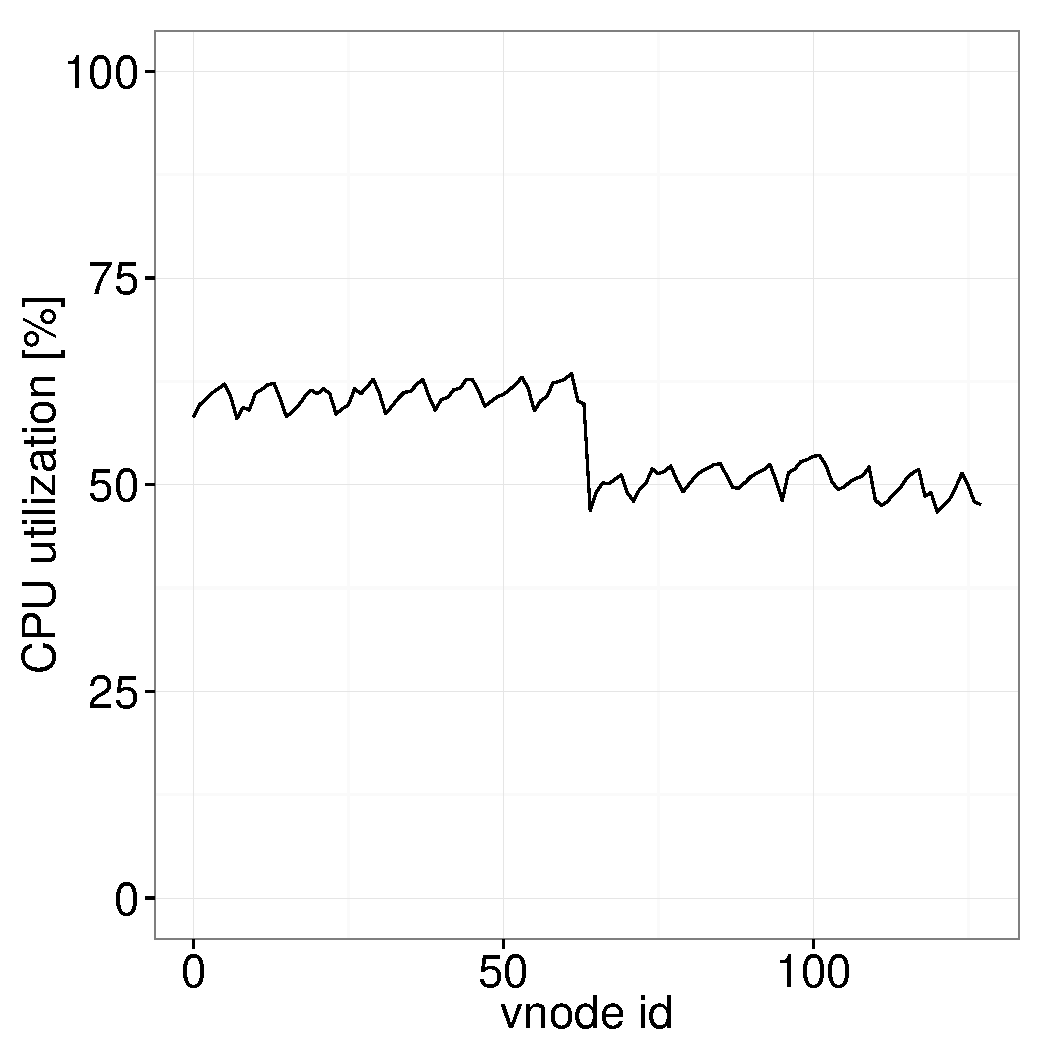
\includegraphics[scale=0.22,angle=0]{figures/usage-heterogeneous.pdf}
    \caption{\centering LBOff \newline Walltime: 341 secs}
    \label{fig:heterogeneous}
\end{figure}
    \end{center}\end{minipage}\hfill
\begin{minipage}{0.3\textwidth}
    \begin{center}
\begin{figure}
    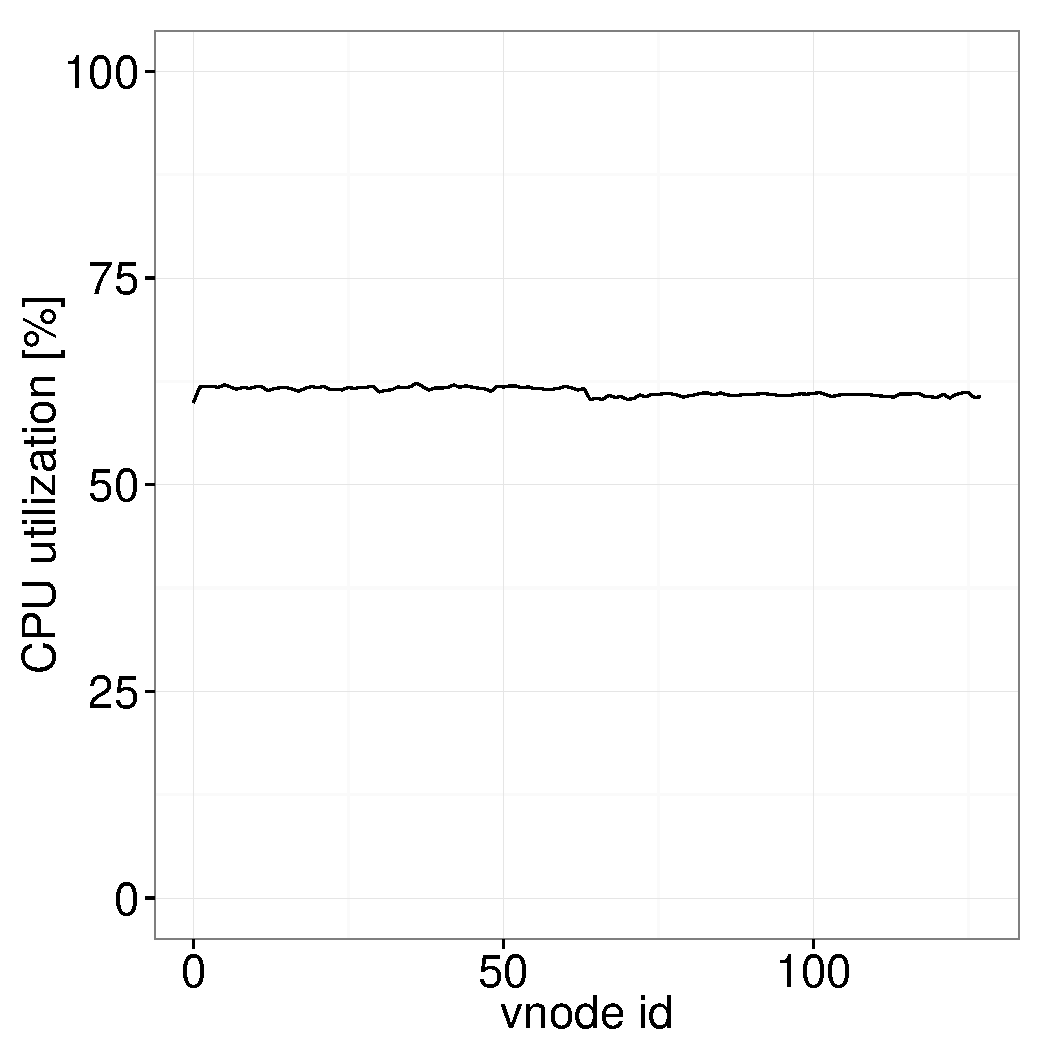
\includegraphics[scale=0.22,angle=0]{figures/usage-heterogeneous_refinelb.pdf}
   \caption{\centering RefineLB \newline Walltime: 320 secs}
    \label{fig:refinelbh}
\end{figure}
\end{center}\end{minipage}\hfill
    \begin{minipage}{0.3\textwidth}
    \begin{center}
\begin{figure}
    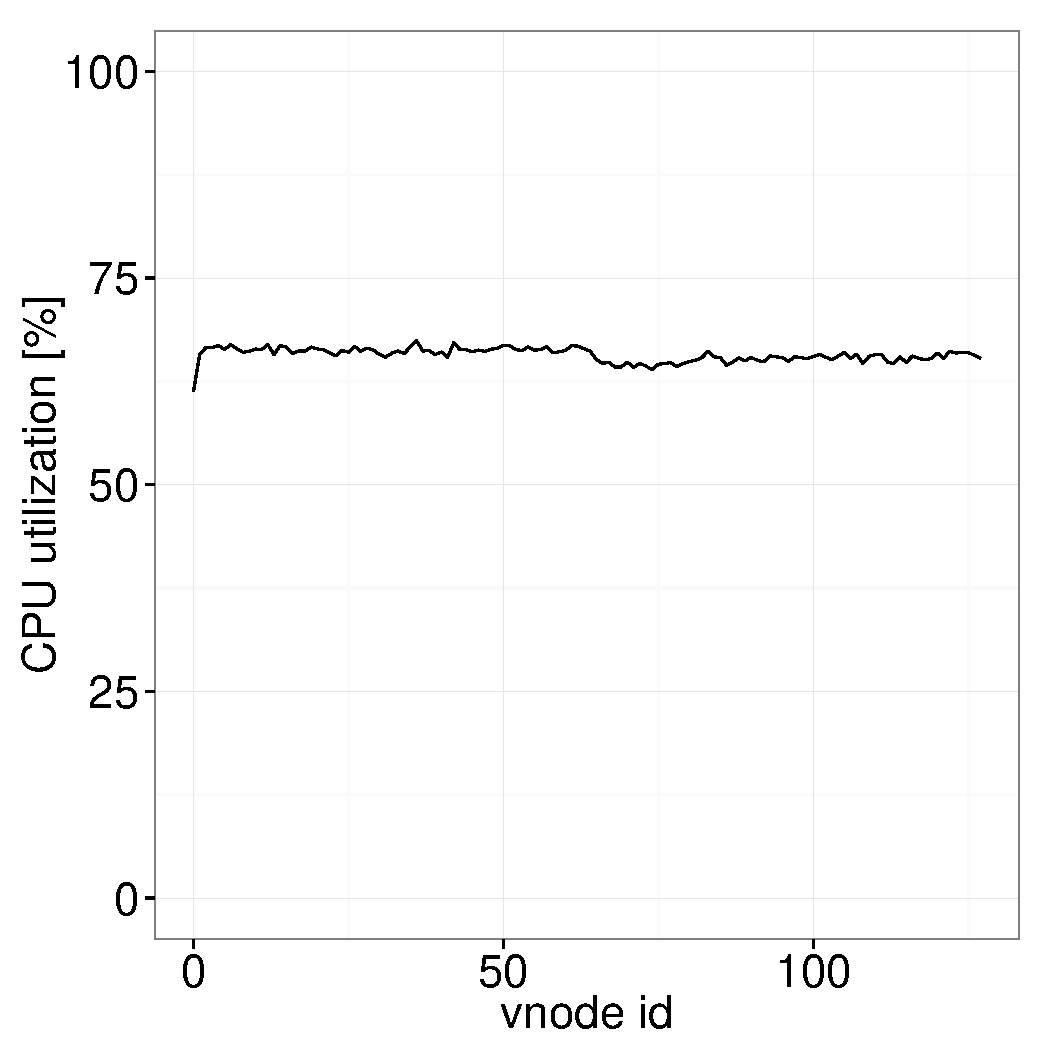
\includegraphics[scale=0.22,angle=0]{figures/usage-heterogeneous_hybrid}
    \caption{\centering Hybrid \newline Walltime: 356 secs}
        \label{fig:hybridlbh}
\end{figure}
    \end{center}\end{minipage}
\end{frame}

\begin{frame}[label=sec-3-0-12]{Evaluating load balancing strategies in Charm++}
Running Stencil3D using 128 processes in the dynamic platform

\vspace{0.5cm}
\begin{minipage}{0.30\textwidth}
\begin{center}
\begin{figure}
    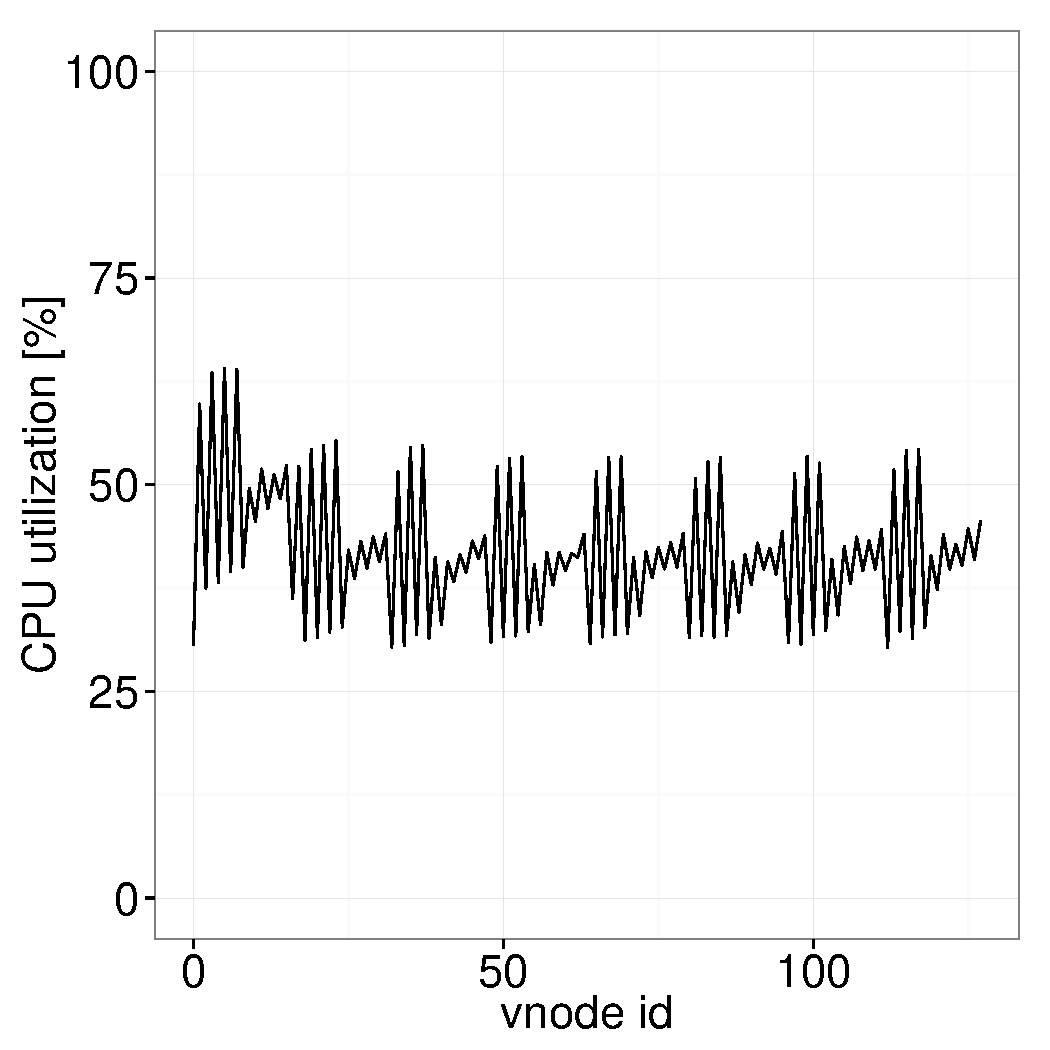
\includegraphics[scale=0.22,angle=0]{figures/usage-dynamic}
    \caption{\centering LBOff \newline Walltime: 347 secs}
    \label{fig:heterogeneous}
\end{figure}
    \end{center}\end{minipage}\hfill
\begin{minipage}{0.3\textwidth}
    \begin{center}
\begin{figure}
    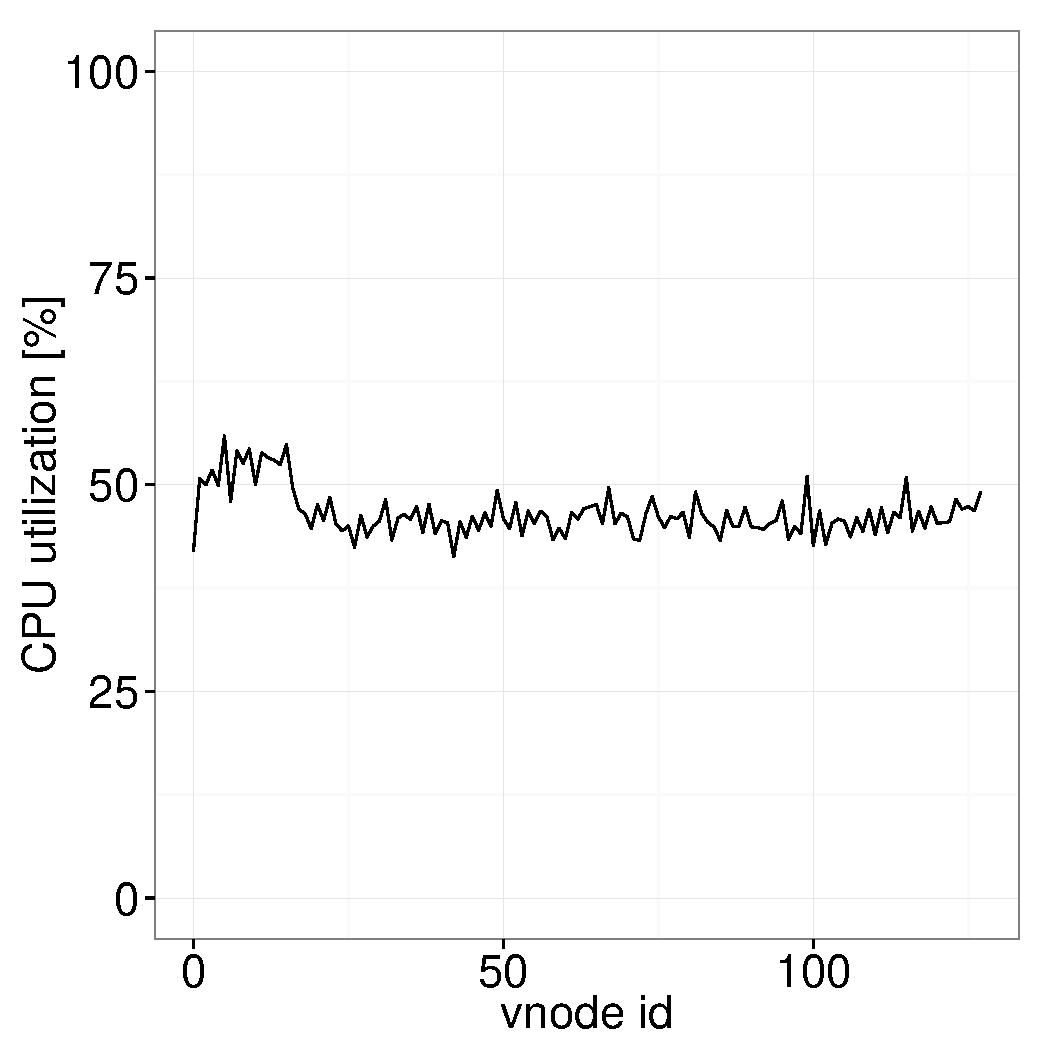
\includegraphics[scale=0.22,angle=0]{figures/usage-dynamic_refinelb}
   \caption{\centering RefineLB \newline Walltime: 322 secs}
    \label{fig:refinelbh}
\end{figure}
\end{center}\end{minipage}\hfill
    \begin{minipage}{0.3\textwidth}
    \begin{center}
\begin{figure}
    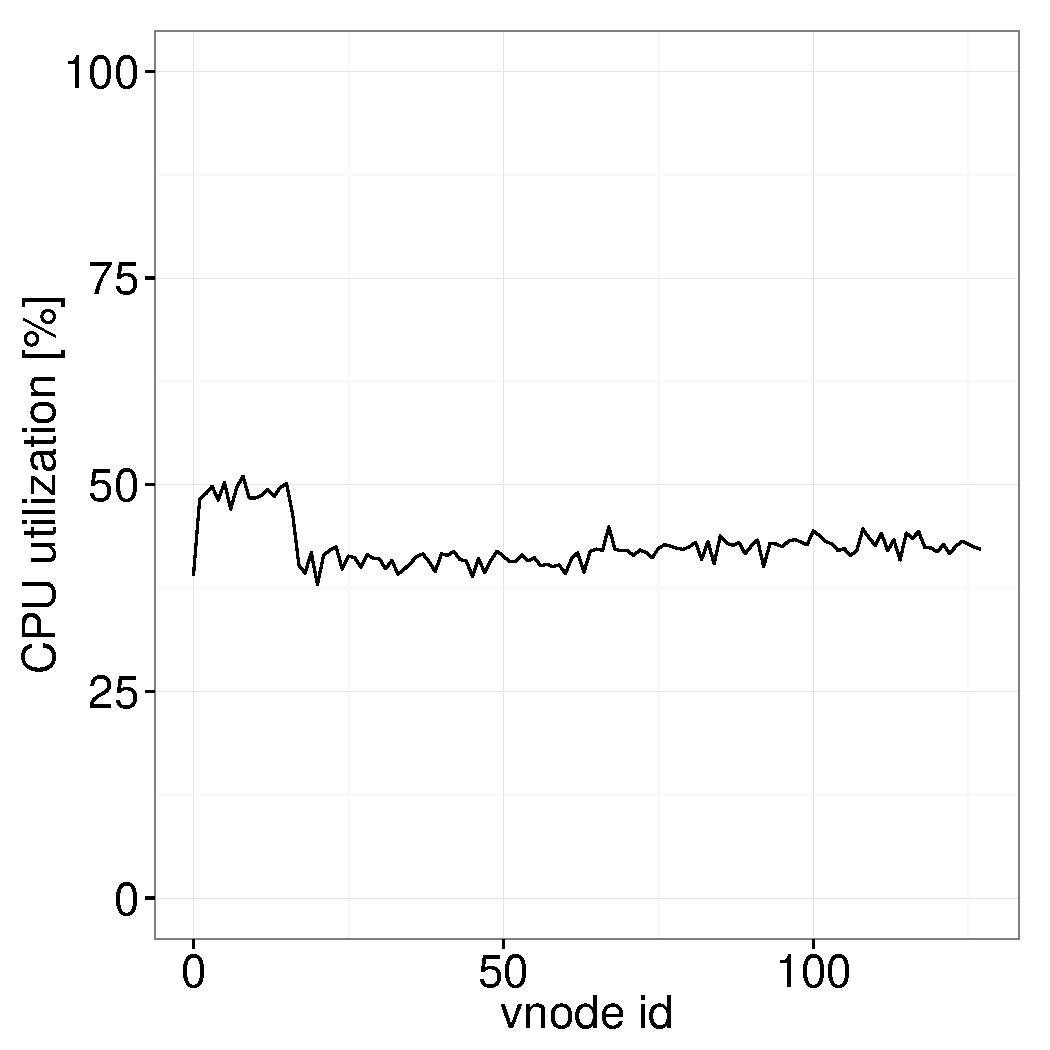
\includegraphics[scale=0.22,angle=0]{figures/usage-dynamic_hybrid}
    \caption{\centering Hybrid \newline Walltime: 359 secs}
        \label{fig:hybridlbh}
\end{figure}
    \end{center}\end{minipage}
\end{frame}

\section{Distem valildation for HPC applications}
\label{sec-4}
\begin{frame}[label=sec-4-0-1]{Containers}
\alert{Containers} refers generally to \alert{Operating-system-level virtualization},
 where the \alert{kernel} of an operating system allows for multiple isolated \alert{user-space instances}.

\begin{figure}[!h]
  \center
  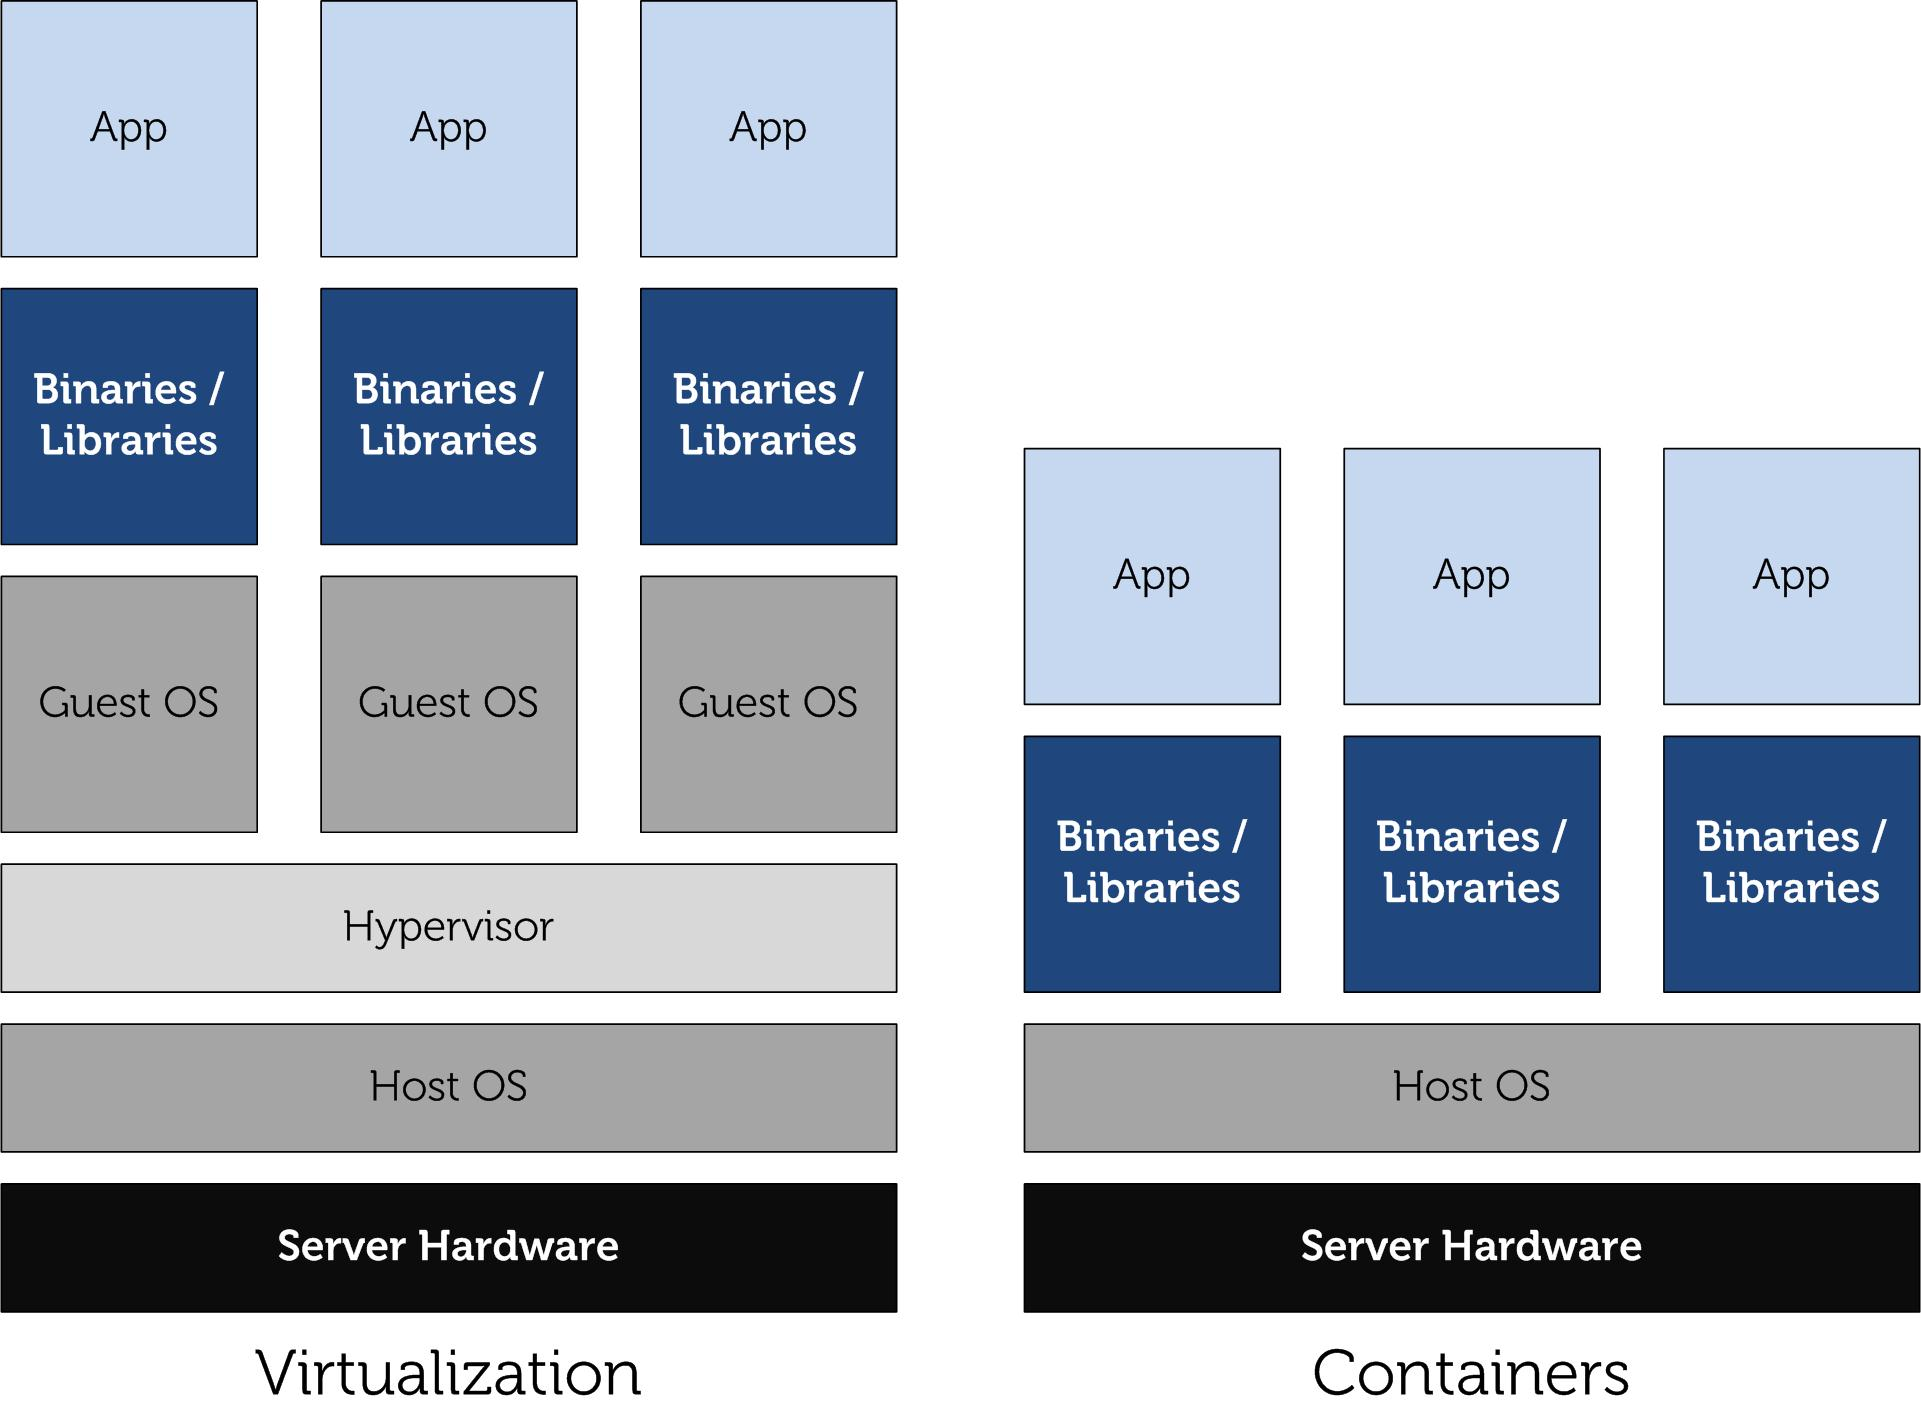
\includegraphics[scale=0.65]{figures/lxc-vm.jpg}
  \label{fig:hpc}
\end{figure}
\end{frame}

\begin{frame}[label=sec-4-0-2]{\emph{namespaces and cgroups}}
\begin{itemize}
\item Both features incorporated in Linux kernel since 2006 (Linux 2.6.24)
\item Several container solutions: LXC, libvirt, libcontainer, systemd-nspawn, Docker
\end{itemize}

\begin{figure}[!h]
  \center
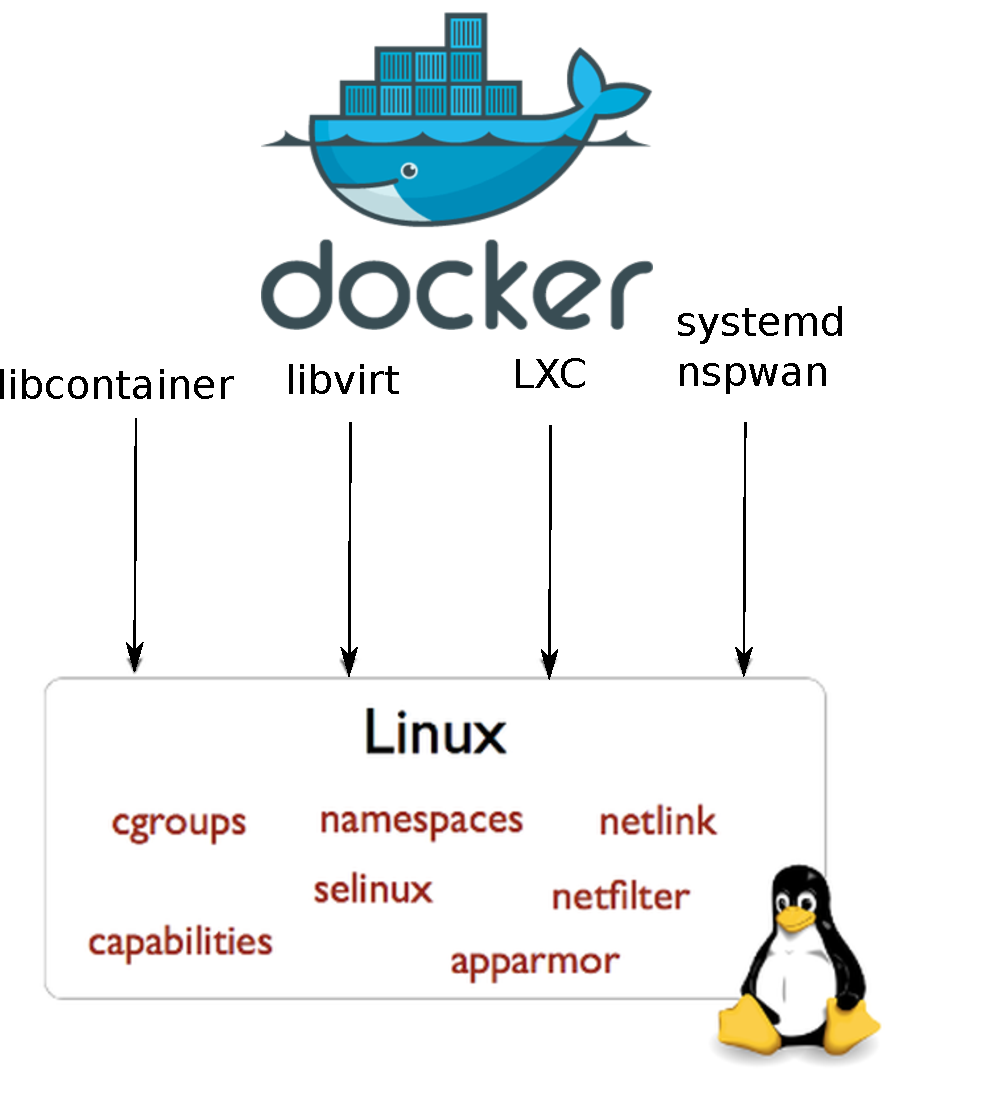
\includegraphics[scale=0.30]{figures/libcontainer-diagram.pdf}
  \label{fig:hpc}
\end{figure}
\end{frame}

\begin{frame}[label=sec-4-0-3]{In this task, we answer:}
\begin{itemize}
\item What is the overhead of oversubscription using different versions of Linux kernel?
\end{itemize}
\begin{itemize}
\item What is the impact of running an HPC workload with several MPI processes inside containers?
\item What is the impact of network technology ?
\end{itemize}
\end{frame}

\begin{frame}[label=sec-4-0-4]{Experimental setup}
\begin{block}{Hardware}
\begin{itemize}
\item Cluster in Grid'5000 Testbed where each node is equipped
with two Intel Xeon E5-2630v3 processors (with 8 cores each), 128 GB of RAM and a 10 GbE adapter
\item Our experimental setup included up to 64 machines
\end{itemize}
\end{block}

\begin{block}{Software}
\begin{itemize}
\item Debian Jessie, Linux kernel versions: 3.2, 3.16 and 4.0, OpenMPI and NPB.
We instrumented the benchmarks: LU, EP, CG, MG, FT, IS using TAU
\end{itemize}
\end{block}
\end{frame}


\begin{frame}[label=sec-4-0-5]{Network setup}
\begin{itemize}
\item \alert{Veth pair + Linux bridge}
\item Veth pair + OpenvSwitch
\item MACVLAN or SR-IOV
\item Phys
\end{itemize}

\begin{figure}[!h]
  \center
  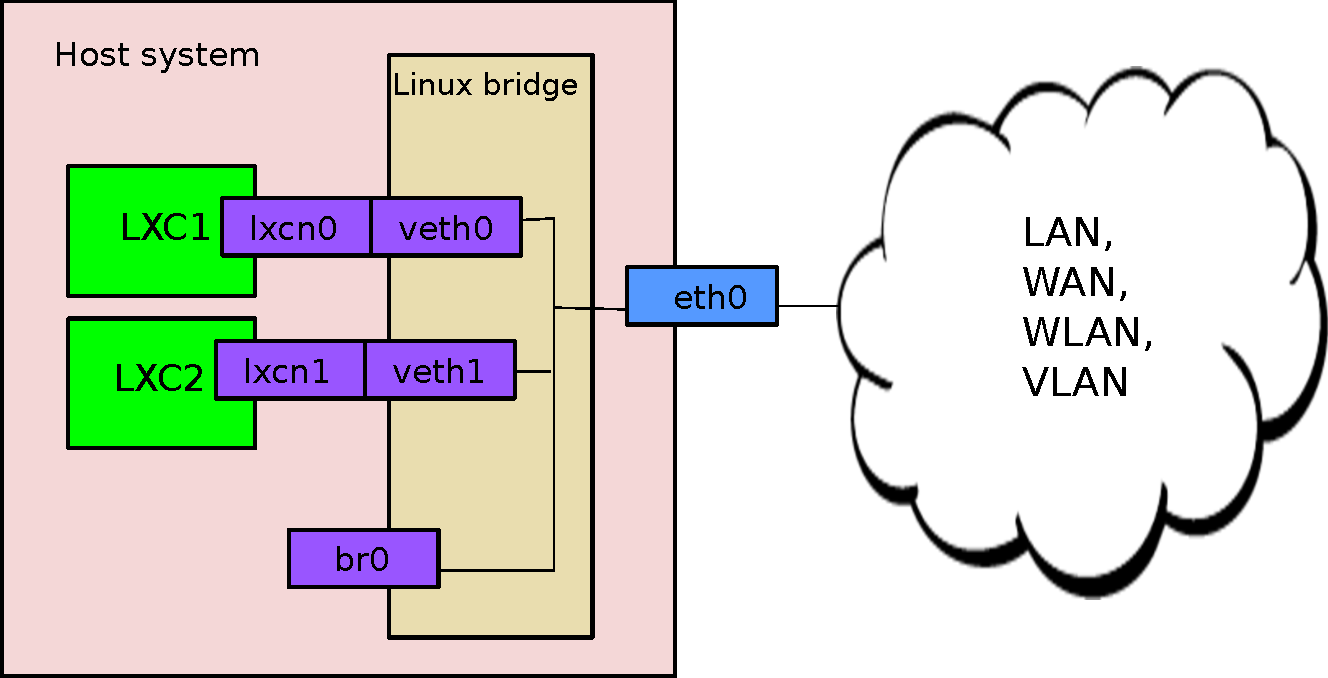
\includegraphics[scale=0.4]{figures/lxc-veth.pdf}
  \label{fig:hpc}
\end{figure}
\end{frame}

\begin{frame}[label=sec-4-0-6]{Linux kernel version}
32 containers running on: 8,16,32 physical machines.

\begin{columns}
\begin{column}{0.5\textwidth}
\begin{block}{Results}

\begin{itemize}
\item 2/node
\begin{itemize}
\item 3.2: \alert{1577.78\%}
\item 3.16: \alert{22.67\%}
\item 4.0: \alert{2.40\%}
\end{itemize}
\item Overhead present in MPI communication
\item Since Linux kernel version \alert{3.11}, \alert{TSO} was enabled in \alert{veth}
\end{itemize}
\end{block}
\end{column}


\begin{column}{0.5\textwidth}





\begin{figure}[!h]
  \center
  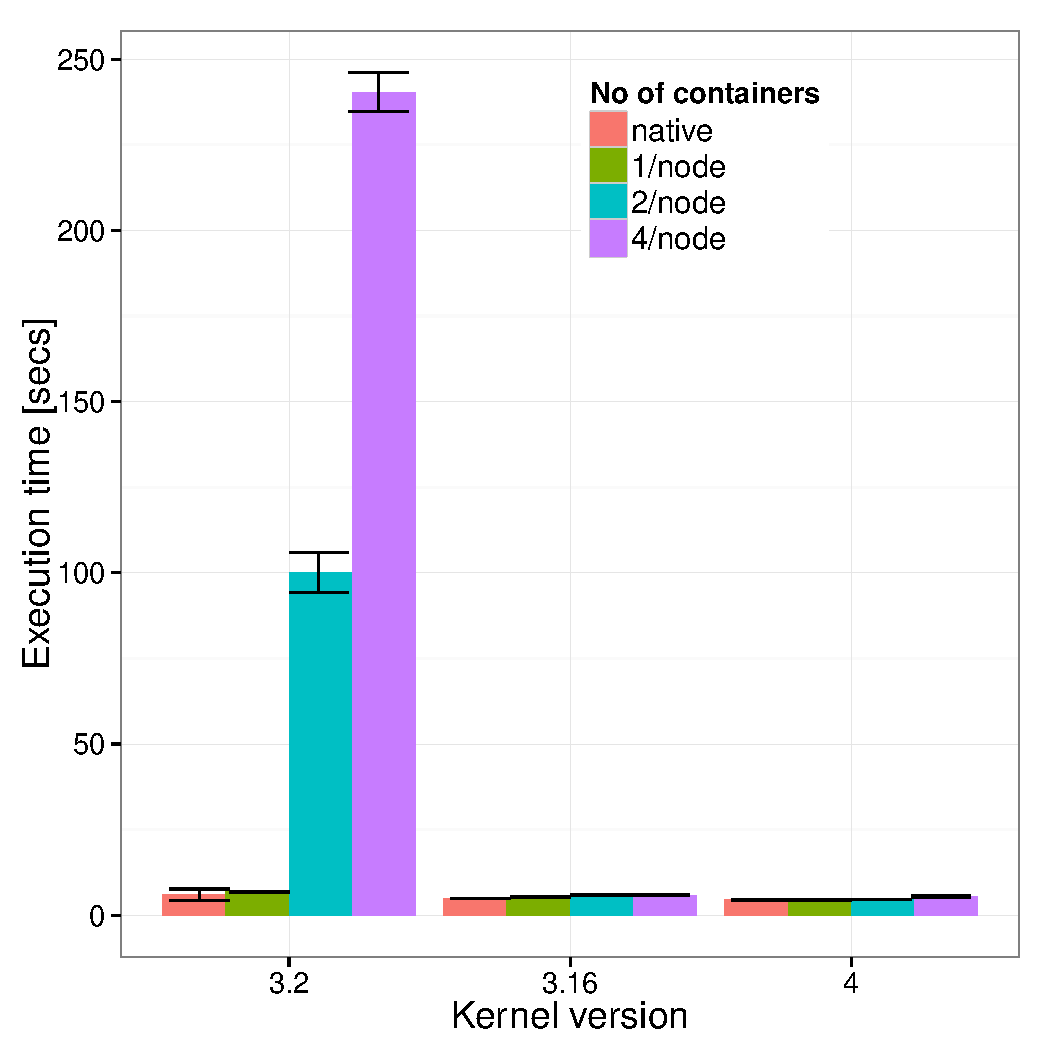
\includegraphics[scale=0.32]{figures/execution_time-kernel-cgB.pdf}
  \label{fig:hpc}
  \caption{CG.B}
\end{figure}
\end{column}
\end{columns}
\end{frame}

\begin{frame}[label=sec-4-0-7]{Multinode inter-container communication}
\begin{itemize}
\item 16 MPI processes were run per physical machine or container
\item We used a maximum of 32 physical machines
\end{itemize}

\begin{figure}
  \centering
  \begin{subfigure}[b]{0.42\textwidth}
    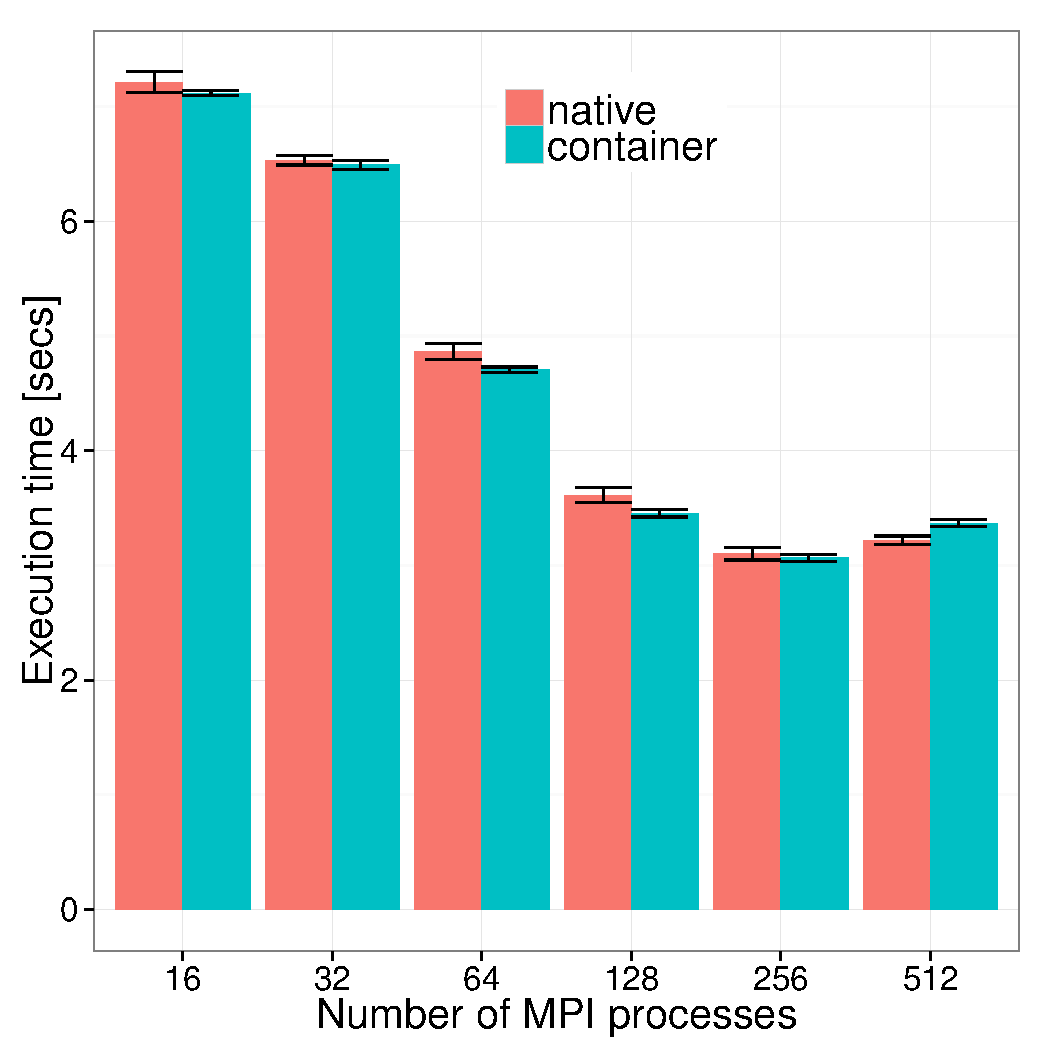
\includegraphics[scale=0.25,angle=0]{figures/veth_overhead-tso-ftB.pdf}
    \caption{FT Class B}
  \end{subfigure}
  \begin{subfigure}[b]{0.42\textwidth}
    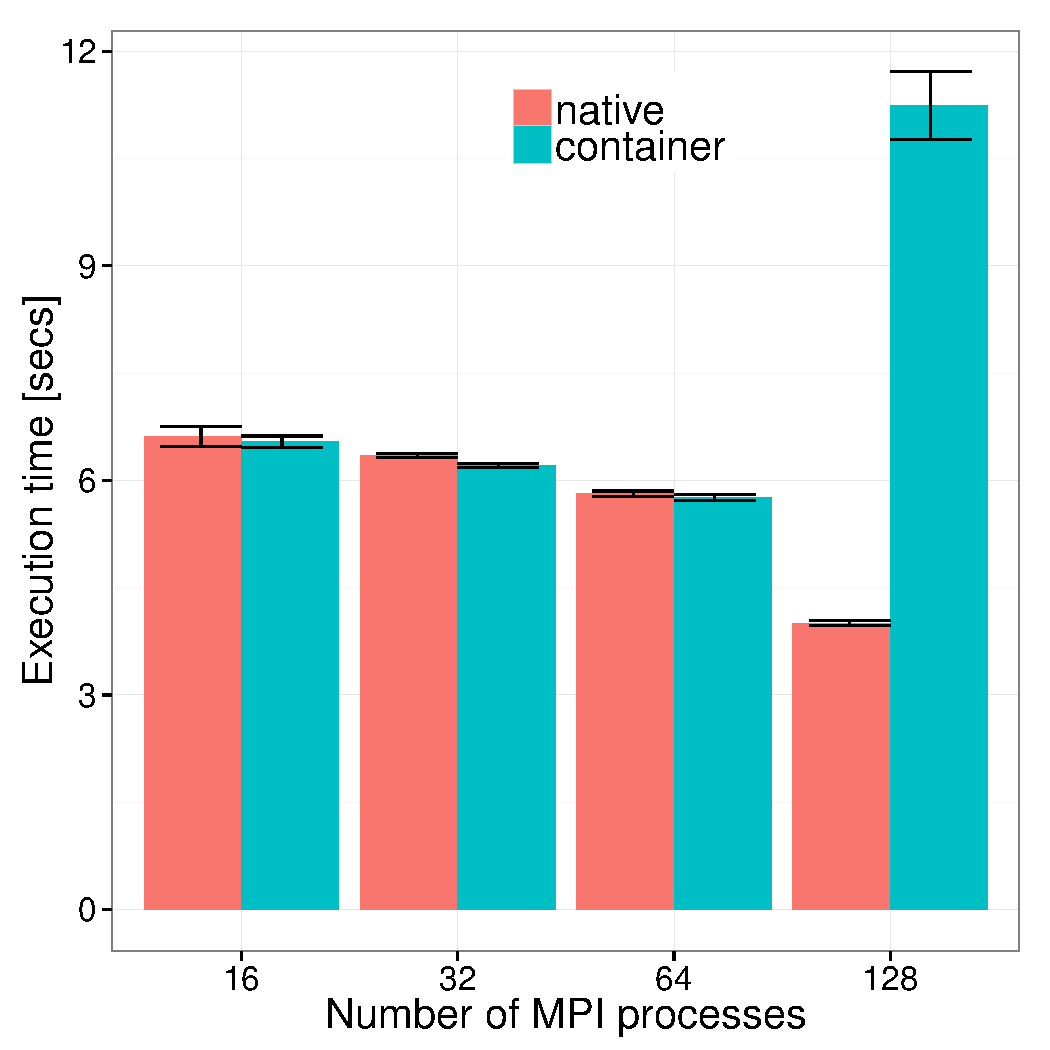
\includegraphics[scale=0.25,angle=0]{figures/veth_overhead-tso-cgB.pdf}
    \caption{CG Class B}
  \end{subfigure}
\end{figure}
\end{frame}

\begin{frame}[label=sec-4-0-8]{Interconnection comparison}
\begin{itemize}
\item \alert{Veth pair + Linux bridge}
\item \alert{Veth pair + OpenvSwitch}
\item \alert{SR-IOV}
\item Using Linux kernel 4.3
\end{itemize}

\begin{figure}[!h]
  \center
  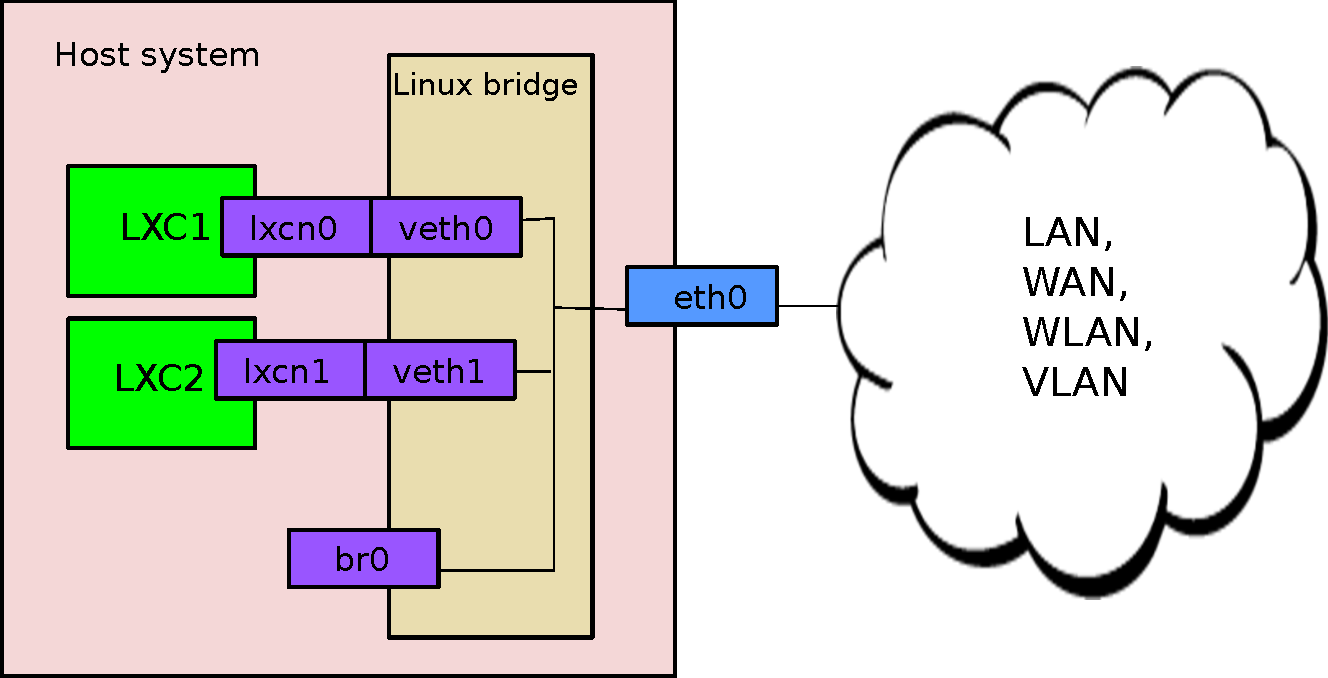
\includegraphics[scale=0.4]{figures/lxc-veth.pdf}
  \label{fig:hpc}
\end{figure}
\end{frame}

\begin{frame}[label=sec-4-0-9]{SR-IOV explained}
\begin{itemize}
\item \alert{Veth pair + Linux bridge}
\item \alert{Veth pair + OpenvSwitch}
\item \alert{SR-IOV}
\end{itemize}

\begin{figure}[!h]
  \center
  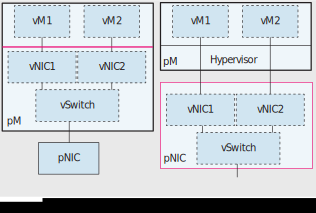
\includegraphics[scale=0.8]{figures/SR-IOV.pdf}
\end{figure}
\end{frame}

\begin{frame}[label=sec-4-0-10]{One machine (intra-node communication)}
\begin{itemize}
\item 1 MPI process per container
\item 16 containers in total
\end{itemize}

\begin{figure}
  \centering
  \begin{subfigure}[b]{0.42\textwidth}
    \caption{FT Class B}
    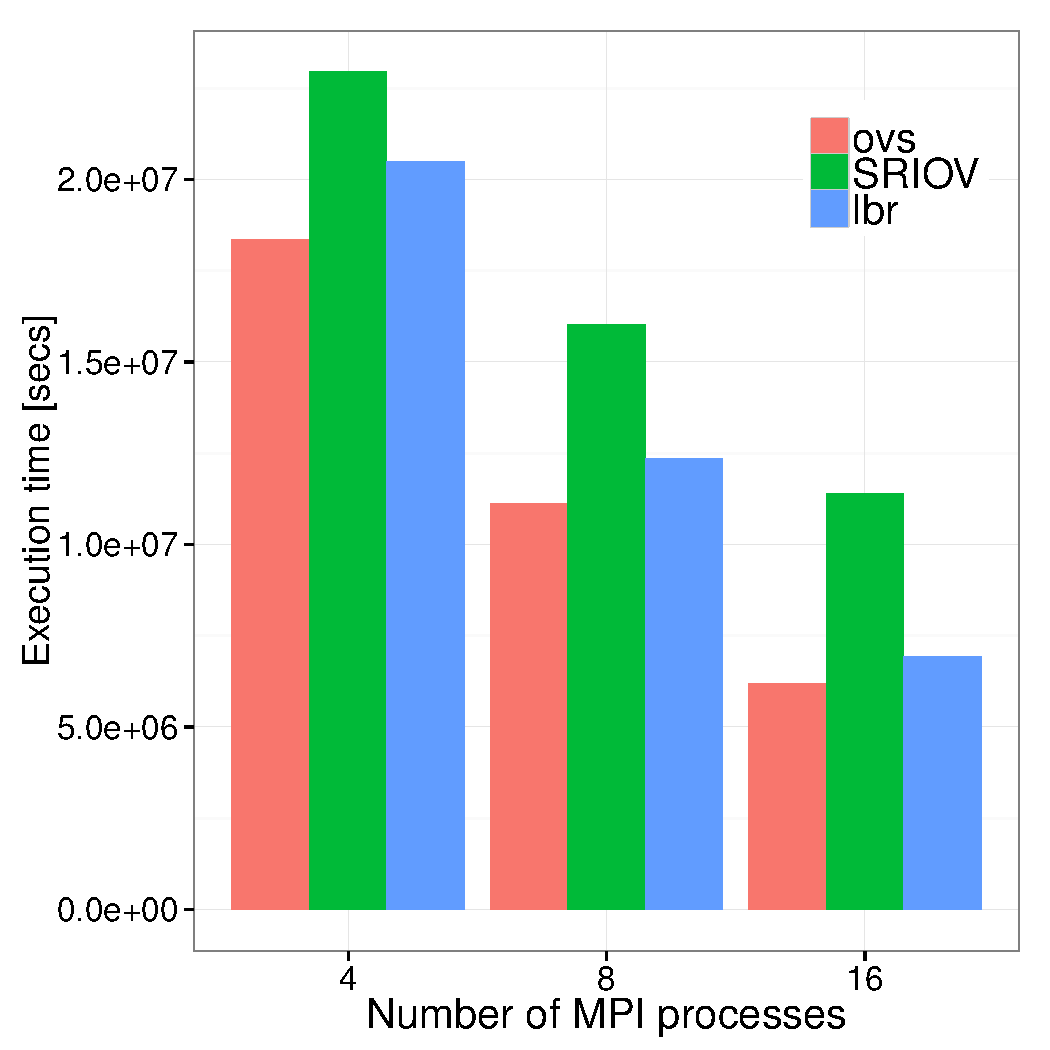
\includegraphics[scale=0.25,angle=0]{figures/intra-container-ftB.pdf}
  \end{subfigure}
  \begin{subfigure}[b]{0.42\textwidth}
    \caption{EP Class B}
    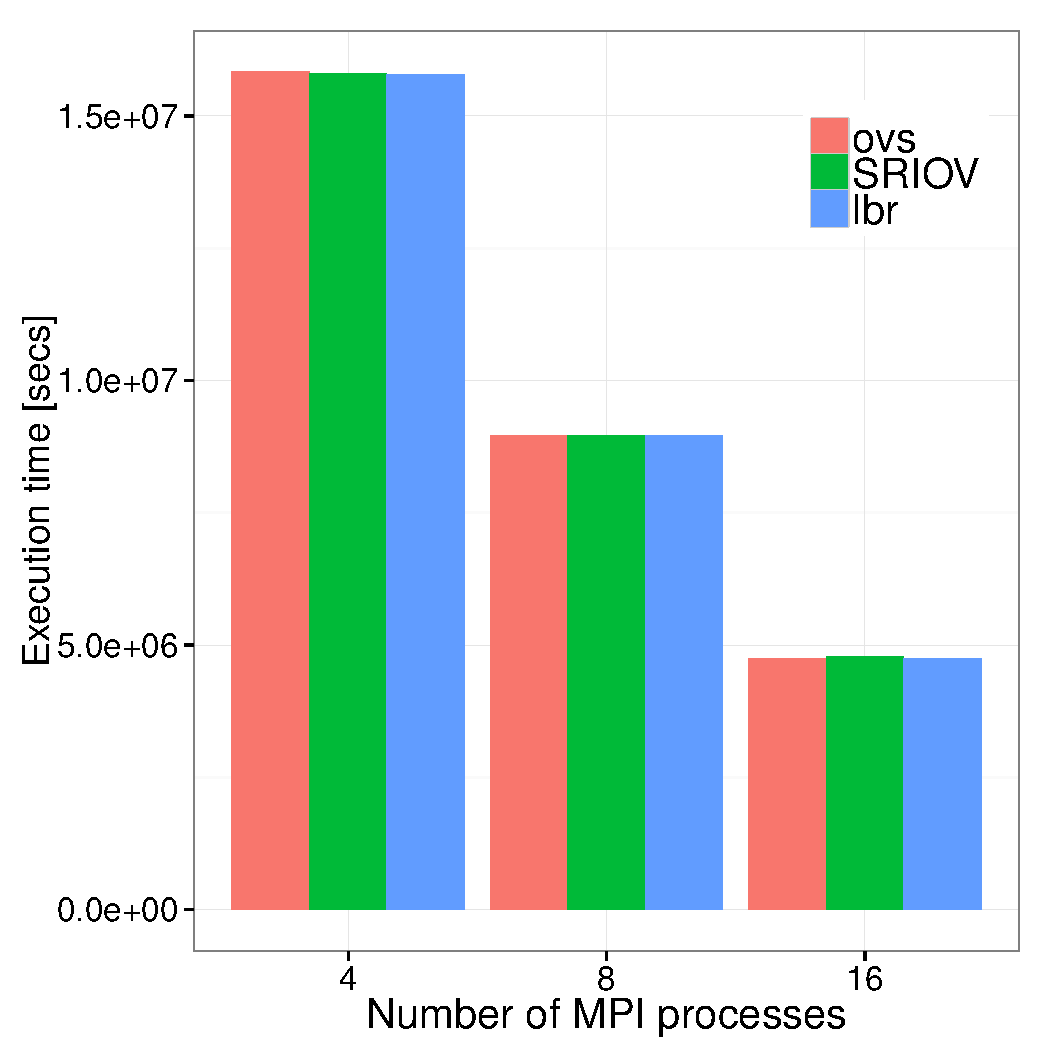
\includegraphics[scale=0.25,angle=0]{figures/intra-container-epB.pdf}
  \end{subfigure}
\end{figure}
\end{frame}

\begin{frame}[label=sec-4-0-11]{Multi-machine (4 nodes)}
\begin{itemize}
\item 4 containers per machine
\item Each container configured with 4 cores
\end{itemize}

\begin{figure}
  \centering
  \begin{subfigure}[b]{0.42\textwidth}
    \caption{LU Class B}
    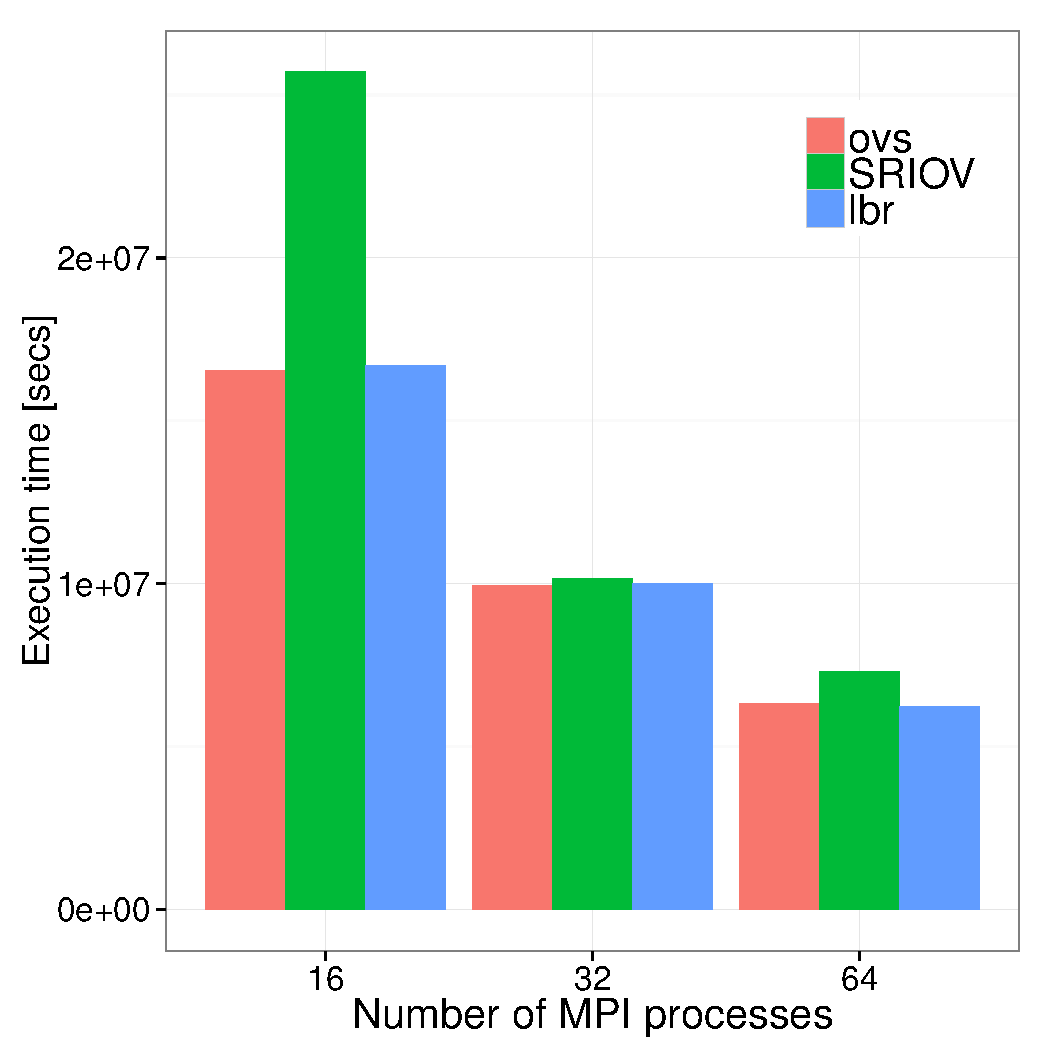
\includegraphics[scale=0.25,angle=0]{figures/inter-container-luB.pdf}
  \end{subfigure}
  \begin{subfigure}[b]{0.42\textwidth}
    \caption{EP Class B}
    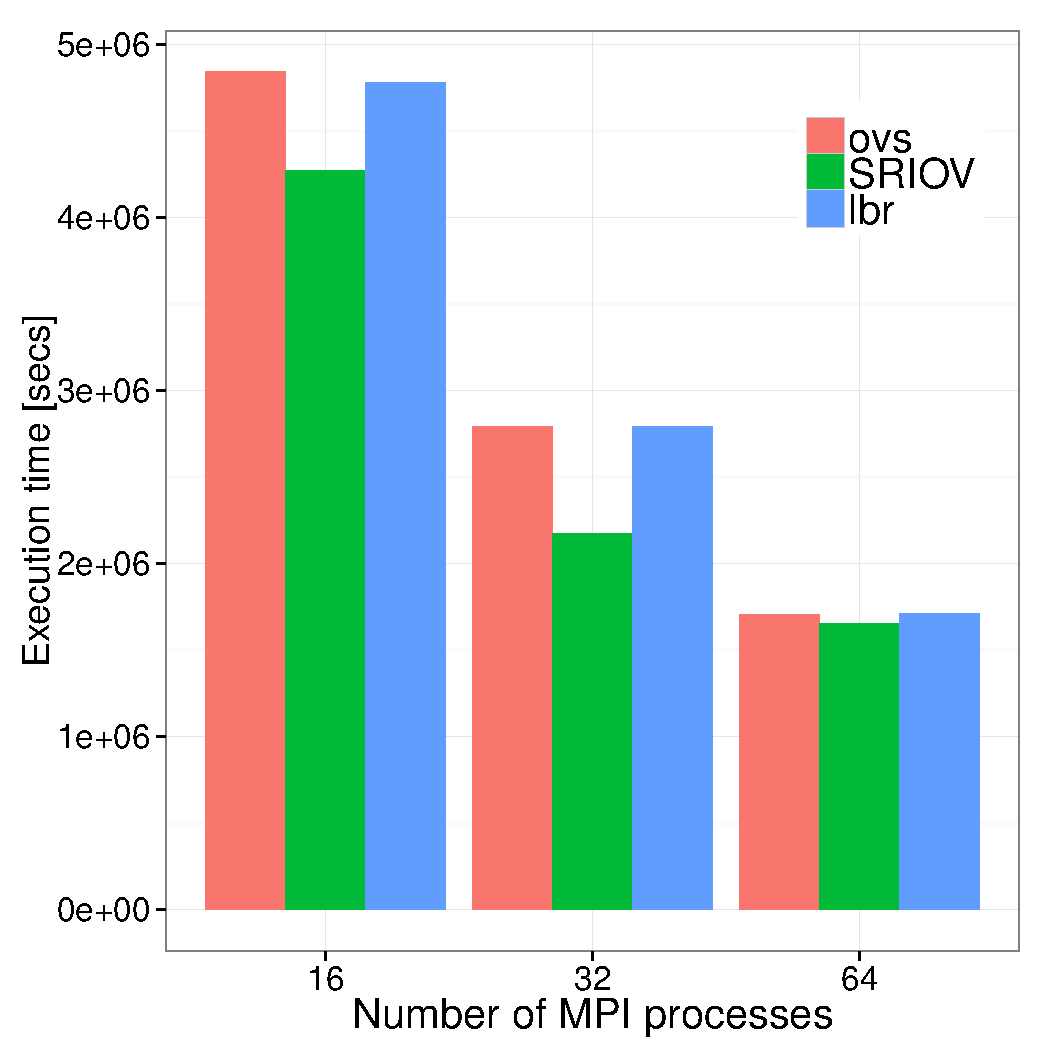
\includegraphics[scale=0.25,angle=0]{figures/inter-container-epB.pdf}
  \end{subfigure}
\end{figure}
\end{frame}

\begin{frame}[label=sec-4-0-12]{Multi-machine (4 nodes other topology)}
\begin{itemize}
\item 4 containers per machine
\item Each container configured with 4 cores
\end{itemize}


\begin{figure}
  \centering
  \begin{subfigure}[b]{0.42\textwidth}
    \caption{LU Class B}
    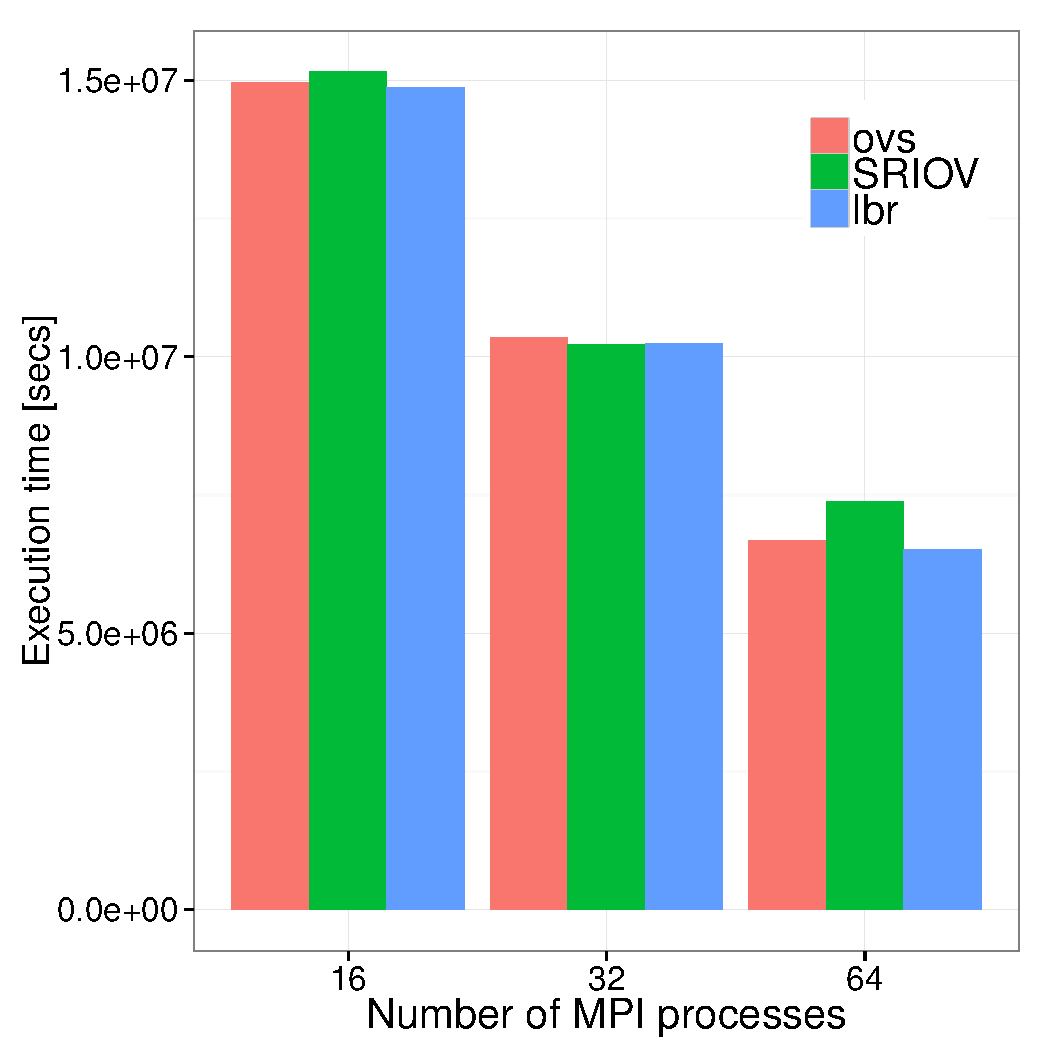
\includegraphics[scale=0.25,angle=0]{figures/inter-container-topo-luB.pdf}
    \label{fig:epkernelversion}
  \end{subfigure}
  \begin{subfigure}[b]{0.32\textwidth}
    \caption{EP Class B}
    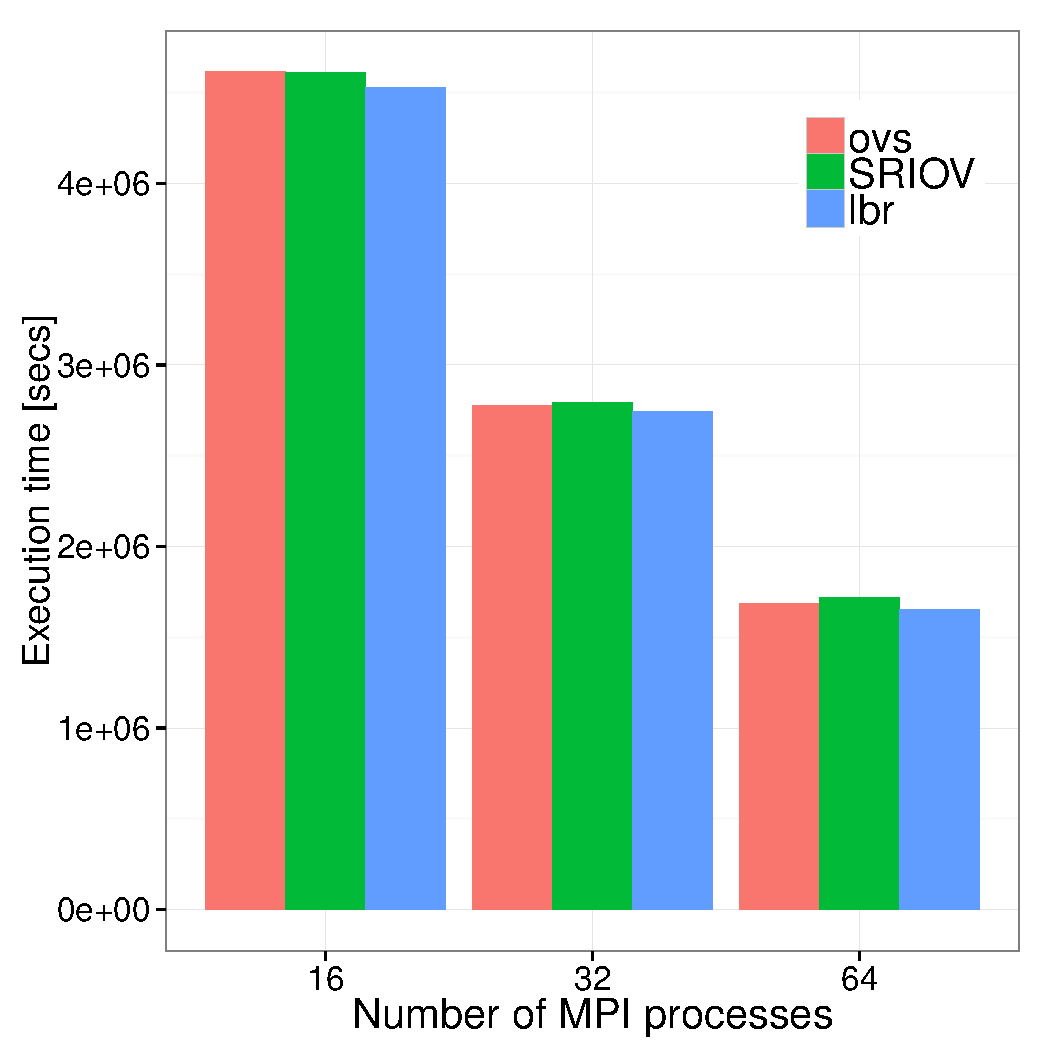
\includegraphics[scale=0.25,angle=0]{figures/inter-container-topo-epB.pdf}
\label{fig:lukernelversion}
  \end{subfigure}
\end{figure}
\end{frame}
\section{Demo time}
\label{sec-5}
\begin{frame}[label=sec-5-0-1]{Docker}
It's time for a \href{https://github.com/alegrand/RR_webinars/blob/master/2_controling_your_environment/docker-tutorial.org}{Docker Demo} (follow the links from
\url{https://github.com/alegrand/RR_webinars/})

Docker advantages for reproducible research:

\begin{itemize}
\item Integrating into local development environments
\item Modular reuse
\item Portable environments
\item Public repositories for sharing
\item Versioning
\end{itemize}

\bottomcite{Carl Boettiger,
   \href{http://www.carlboettiger.info/assets/files/pubs/10.1145/2723872.2723882.pdf}{\textit{An introduction to Docker for reproducible research}},
  ACM SIGOPS Operating Systems Review,2015}
\end{frame}

\begin{frame}[fragile,label=sec-5-0-2]{Docker advantages}
 \begin{itemize}
\item Portable computation \& sharing
\end{itemize}

\begin{minted}[frame=lines,fontsize=\scriptsize,linenos]{sh}
$ docker export container-name > container.tar
$ docker push username/r-recommended
\end{minted}

\begin{itemize}
\item Re-usable modules
\end{itemize}
\begin{minted}[frame=lines,fontsize=\scriptsize,linenos]{sh}
$ docker run -d --name db training/postgres
$ docker run -d -P --link db:bd training/webapp \
   python app.py
\end{minted}

\begin{itemize}
\item Versioning
\end{itemize}

\begin{minted}[frame=lines,fontsize=\scriptsize,linenos]{sh}
$ docker history r-base
$ docker tag  d7e5801bb7ac ttimbers/mmp-dyf-skat:latest
\end{minted}
\end{frame}

\section{Conclusions}
\label{sec-6}
\begin{frame}[label=sec-6-0-1]{Conclusions}
\begin{itemize}
\item Being able to execute experiments on a large set of platform
configurations in a repeatable way is a sound basis to design
and improve the HPC runtimes in the future
\end{itemize}

\vspace{0.5cm}
\begin{itemize}
\item \alert{Distem:}
\begin{itemize}
\item offers realistic experimental conditions

\item simplified the uncovering of problems in the
failure handling for widely used HPC runtimes

\item enables experimenters to easily simulate perturbations and
heterogeneity of nodes
\end{itemize}
\end{itemize}
\end{frame}
\begin{frame}[label=sec-6-0-2]{What did we find?}
\begin{itemize}
\item There is important performance degradation provoked by \alert{veth} for Linux kernels < 3.11
\item Container placing plays in important role under oversubscription
\item Memory bound applications and application that use \alert{all to all MPI} communication are
the most affected by oversubscription
\end{itemize}
\end{frame}

\begin{frame}[label=sec-6-0-3]{What is next}
\begin{itemize}
\item Adapt Distem to SDN and NDN needs
\item Integrate: \emph{time dilation}
\end{itemize}
\end{frame}
% Emacs 24.3.1 (Org mode 8.2.10)
\end{document}
